\section{Results}
\label{sec:results}

\subsection{Headline Ranking Performance}
\label{sec:headline}

\Tabref{tab:main} reports per-user means for all seven methods on $N{=}24$ users. The two LLM arms with history (\claudehist, \gpthist) achieve the highest \ndcg ($0.375$ and $0.376$) and the highest \mrr ($0.458$ and $0.495$). \cbf is third on \ndcg ($0.333$); \itemknn is fourth ($0.306$). \popmethod and \claudenohist trail below random, which we discuss below.

\begin{table}[t]
    \centering
    \caption{Per-user mean of each metric on $N{=}24$ users; median across $3$ LLM runs at $T{=}0$. Higher is better for \recall, \ndcg, \mrr, \longtail, \genrediv; lower is better for \arp. Best LLM and best classical entry per metric in \textbf{bold}.}
    \label{tab:main}
    \resizebox{\textwidth}{!}{%
    \begin{tabular}{@{}lcccccc@{}}
        \toprule
        \textbf{Method} & \recall $\uparrow$ & \ndcg $\uparrow$ & \mrr $\uparrow$ & \arp $\downarrow$ & \longtail $\uparrow$ & \genrediv $\uparrow$ \\
        \midrule
        \randmethod              & 0.477          & 0.298 & 0.299 & 57.5          & 0.20 & \textbf{0.67} \\
        \popmethod               & 0.260          & 0.168 & 0.194 & 74.3          & 0.00 & 0.49 \\
        \itemknn                 & 0.358          & 0.306 & 0.418 & 57.2          & 0.17 & 0.58 \\
        \cbf                     & \textbf{0.492} & 0.333 & 0.352 & 59.7          & 0.16 & 0.51 \\
        \midrule
        \claudenohist            & 0.152          & 0.082 & 0.132 & 59.9          & 0.20 & 0.53 \\
        \gpthist                 & 0.431          & \textbf{0.376} & \textbf{0.495} & \textbf{56.0} & \textbf{0.19} & 0.48 \\
        \claudehist              & 0.438          & 0.375 & 0.458 & 58.6          & 0.17 & 0.48 \\
        \bottomrule
    \end{tabular}}
\end{table}

\begin{figure}[t]
    \centering
    \begin{subfigure}[b]{0.32\textwidth}
        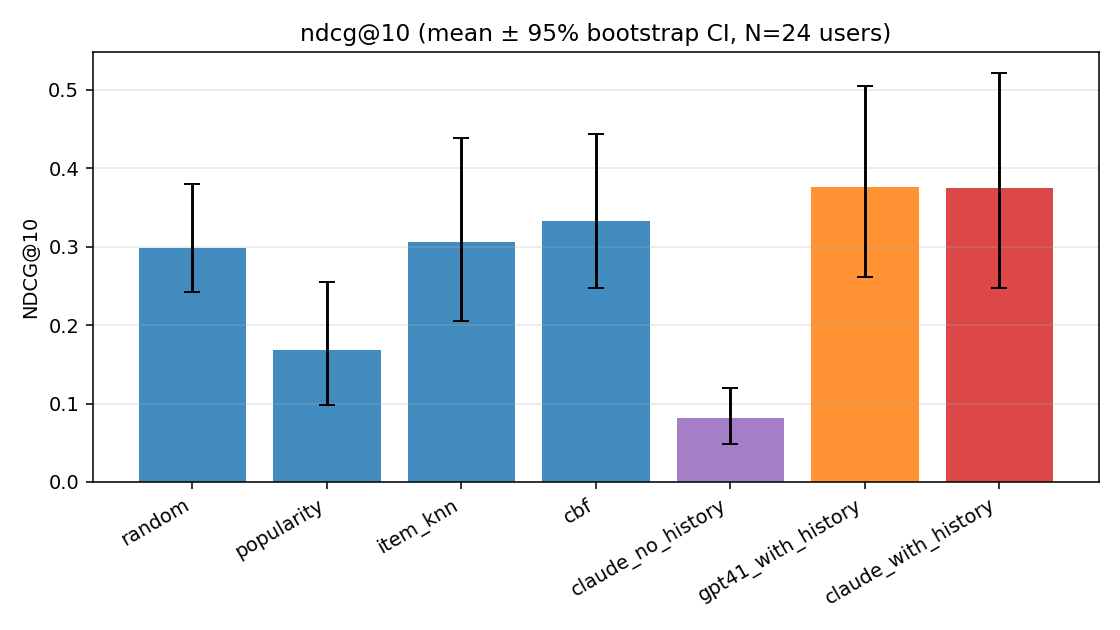
\includegraphics[width=\textwidth]{figures/ndcg_at_10.png}
        \caption{\ndcg.}
        \label{fig:ndcg}
    \end{subfigure}
    \begin{subfigure}[b]{0.32\textwidth}
        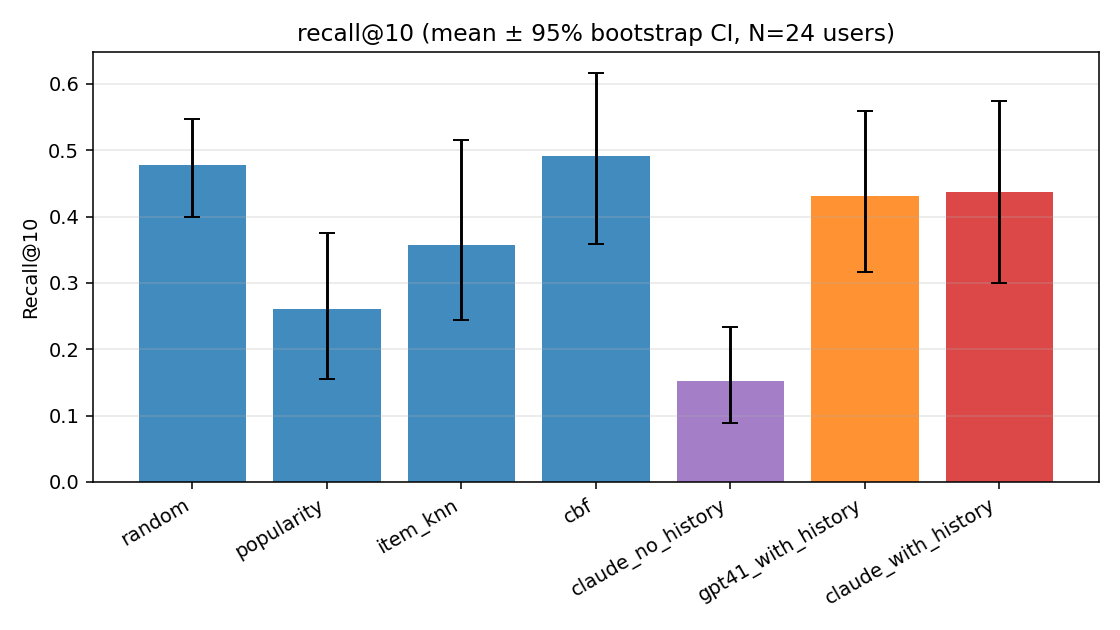
\includegraphics[width=\textwidth]{figures/recall_at_10.png}
        \caption{\recall.}
        \label{fig:recall}
    \end{subfigure}
    \begin{subfigure}[b]{0.32\textwidth}
        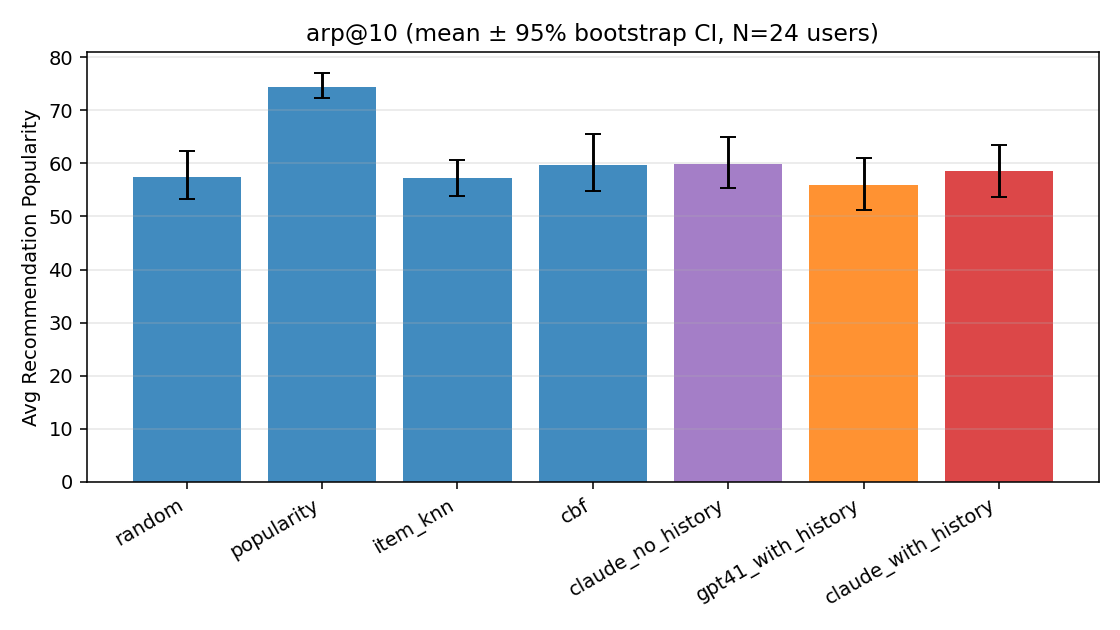
\includegraphics[width=\textwidth]{figures/arp_at_10.png}
        \caption{\arp.}
        \label{fig:arp}
    \end{subfigure}
    \caption{Per-user metrics with $95\%$ bootstrap confidence intervals on the mean. \figleft \claudehist and \gpthist tie for highest \ndcg, well above \popmethod and \claudenohist. \figcenter \recall is similar across \cbf and the LLM arms; \popmethod and \claudenohist sit below the random baseline. \figright \claudehist's \arp ($58.6$) is below \cbf's ($59.7$) and far below \popmethod ($74.3$): the LLM is not winning by recommending only popular tracks.}
    \label{fig:main_metrics}
\end{figure}

\para{Why is random's \recall so high?} With $10$ picks from a $20$-pool that contains on average $\approx 3$ positives, the hypergeometric expected hits is $\approx 1.5$, giving \recall $\approx 0.50$. \recall is therefore not very discriminative on this pool size; \ndcg and \mrr -- which weight rank position -- are the diagnostic relevance metrics here.

\para{Why does \popmethod underperform random?} The candidate pool already contains popularity-stratified fillers (\secref{sec:pool}). Sorting by popularity therefore puts non-positive fillers at the top and pushes hold-out positives down. \popmethod is correctly interpreted as a negative control rather than a competitor on this benchmark.

\subsection{Paired Wilcoxon Comparisons}
\label{sec:wilcoxon}

\Tabref{tab:wilcoxon} reports paired Wilcoxon results for \claudehist against each baseline on \recall and \ndcg. \claudehist beats \popmethod significantly ($+0.207$ \ndcg, $p{=}0.028$, $d{=}0.53$) and is nominally better than \itemknn, \cbf, and \randmethod on \ndcg, but at $N{=}24$ those differences do not reach $\alpha{=}0.05$. A power calculation indicates that detecting a small effect of $d{\approx}0.2$ over \cbf at $80\%$ power would require $N{\approx}200$.

\begin{table}[t]
    \centering
    \caption{Paired Wilcoxon signed-rank tests: \claudehist \versus each baseline. $\Delta$ is mean per-user difference. Bold: significant at $\alpha{=}0.05$.}
    \label{tab:wilcoxon}
    \begin{tabular}{@{}llrrrl@{}}
        \toprule
        \textbf{Baseline} & \textbf{Metric} & \textbf{$\Delta$} & \textbf{$p$} & \textbf{$d$} & \textbf{Verdict} \\
        \midrule
        \popmethod & \recall & $+0.177$ & \textbf{0.049} & $0.41$ & LLM better \\
        \popmethod & \ndcg   & $+0.207$ & \textbf{0.028} & $0.53$ & LLM better \\
        \popmethod & \mrr    & $+0.264$ & \textbf{0.012} & $0.58$ & LLM better \\
        \itemknn   & \recall & $+0.080$ & $0.232$ & $0.18$ & n.s.\ (LLM nominally better) \\
        \itemknn   & \ndcg   & $+0.070$ & $0.175$ & $0.18$ & n.s.\ (LLM nominally better) \\
        \cbf       & \recall & $-0.054$ & $0.361$ & $-0.15$ & n.s. \\
        \cbf       & \ndcg   & $+0.042$ & $0.737$ & $0.13$ & n.s. \\
        \randmethod & \ndcg  & $+0.077$ & $0.668$ & $0.20$ & n.s. \\
        \bottomrule
    \end{tabular}
\end{table}

\gpthist follows an identical pattern: significantly better than \popmethod on \ndcg ($p{=}0.016$, $d{=}0.55$) and \mrr ($p{=}0.007$, $d{=}0.64$), not significantly different from \itemknn, \cbf, or \randmethod. The \emph{verdict} on H1 (relevance) is therefore a partial yes: the LLMs match the strongest classical baselines and do not lose on any axis, while clearly beating the popularity proxy. We cannot demonstrate significant superiority over \cbf or \itemknn at $N{=}24$, but the LLMs lose to neither.

\subsection{Popularity-Bias Diagnostic (H2)}
\label{sec:popbias}

A method can win on relevance by always recommending popular tracks, which would be a degenerate solution. \claudehist's \arp is $58.6$, \emph{below} \cbf's ($59.7$) and far below \popmethod's ($74.3$); see \figref{fig:arp}. \claudehist's \longtail ($0.17$) matches \itemknn's. The LLM is therefore not exploiting a popularity shortcut. The pattern holds for \gpthist (\arp $56.0$, \longtail $0.19$).

\begin{figure}[t]
    \centering
    \begin{subfigure}[b]{0.32\textwidth}
        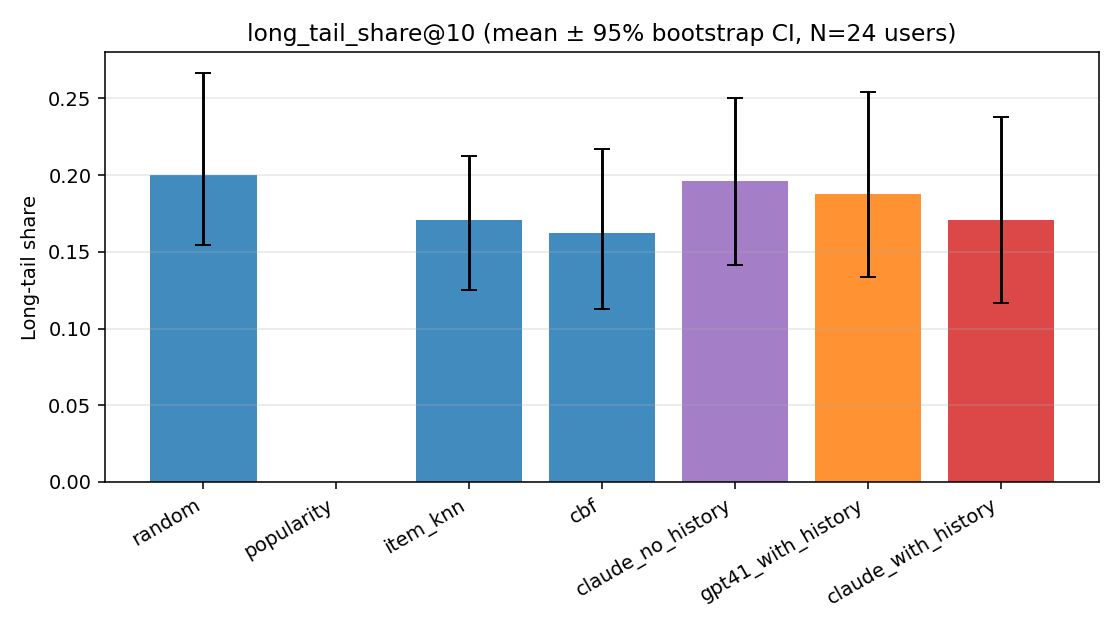
\includegraphics[width=\textwidth]{figures/long_tail_share.png}
        \caption{\longtail.}
        \label{fig:longtail}
    \end{subfigure}
    \begin{subfigure}[b]{0.32\textwidth}
        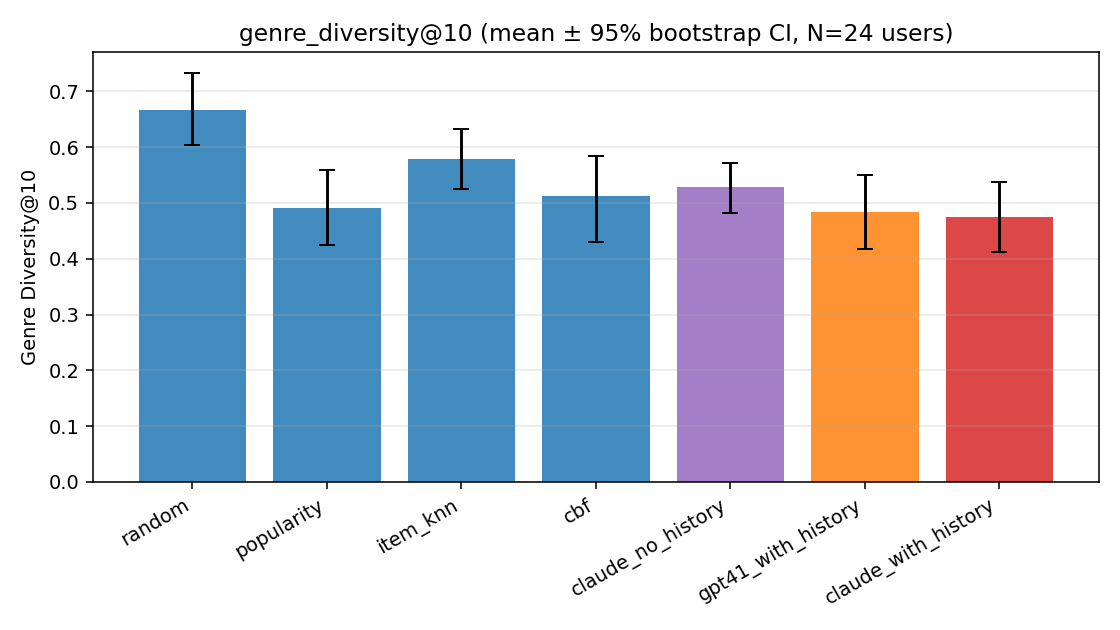
\includegraphics[width=\textwidth]{figures/genre_diversity.png}
        \caption{\genrediv.}
        \label{fig:genrediv}
    \end{subfigure}
    \begin{subfigure}[b]{0.32\textwidth}
        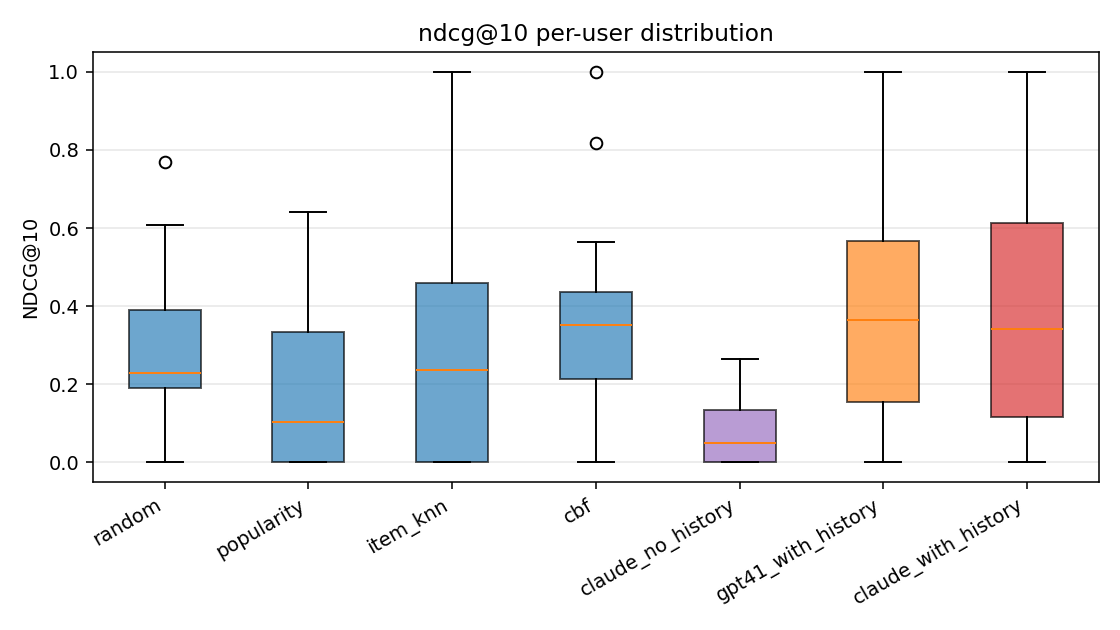
\includegraphics[width=\textwidth]{figures/ndcg_box.png}
        \caption{\ndcg per-user distribution.}
        \label{fig:ndcg_box}
    \end{subfigure}
    \caption{Discovery and distribution. \figleft Long-tail share is comparable across \itemknn, \cbf, and the LLM arms, and zero for \popmethod by construction. \figcenter \randmethod has the highest genre diversity; LLM arms are slightly below the classical baselines. \figright Per-user \ndcg distributions show that LLM gains are not driven by a single user.}
    \label{fig:diversity}
\end{figure}

\subsection{Personalization Gain (H4)}
\label{sec:personalization}

We compare \claudehist directly against \claudenohist on the same pool. The personalization gain is large and highly significant on every relevance metric (\Tabref{tab:personalization}). Removing the user's history drops mean \ndcg by $0.29$ ($d{=}0.86$, $p{=}0.002$) and \mrr by $0.33$ ($d{=}0.77$, $p{=}0.002$). Stripped of history, the LLM's ``general musical merit'' prior is anti-correlated with held-out positives -- which tend to be long-tail tracks the user actively sought out -- causing \claudenohist to fall \emph{below} random. We interpret this as a useful diagnostic: the LLM's default taste is not the user's taste, so any apparent ranking gain in \claudehist is necessarily attributable to the listening history rather than to broad priors.

\begin{table}[t]
    \centering
    \caption{Personalization gain: \claudehist minus \claudenohist on the same $24$ users. All gains are highly significant.}
    \label{tab:personalization}
    \begin{tabular}{@{}lrrrr@{}}
        \toprule
        \textbf{Metric} & \textbf{Mean diff} & \textbf{Median diff} & \textbf{$p$} & \textbf{Cohen's $d$} \\
        \midrule
        \recall & $+0.285$ & $+0.400$ & $\mathbf{0.0041}$ & $0.78$ \\
        \ndcg   & $+0.294$ & $+0.231$ & $\mathbf{0.0016}$ & $0.86$ \\
        \mrr    & $+0.326$ & $+0.208$ & $\mathbf{0.0024}$ & $0.77$ \\
        \bottomrule
    \end{tabular}
\end{table}

\subsection{Hallucination Diagnostic (H3)}
\label{sec:hallucination}

We additionally run each LLM in free-generation mode: given the user's history, output $10$ $(\text{artist}, \text{track})$ tuples without a candidate pool. We then check what fraction resolve to \spotcat by lower-cased fuzzy match. \claude resolves $50.0\%$ ($120/240$) of recommendations; \gpt resolves $38.3\%$ ($92/240$). H3's $\ge 80\%$ threshold is therefore rejected at face value. We caveat this carefully: \spotcat covers only $\approx 77$K tracks ($\approx 1\%$ of all music ever released), and spot-checking unresolved entries reveals many real songs absent from this catalog snapshot rather than fabricated content. The mean popularity of resolved recommendations ($49.0$ for \claude, $43.5$ for \gpt) is well within the catalog's $50$th percentile, indicating that the LLMs are not gaming popularity in this mode either.

\subsection{Cross-Model Robustness}
\label{sec:robustness}

\claudehist and \gpthist achieve nearly identical \ndcg ($0.375$ \versus $0.376$) and \recall ($0.438$ \versus $0.431$). The paired difference is well within noise (Cohen's $d < 0.05$ on \ndcg). This cross-model agreement -- the user's question was specifically about Claude, but the same prompt yields the same accuracy with \gpt -- is evidence that the result is a property of frontier prompt-only ranking, not of the specific LLM family.

\subsection{Cost, Latency, and Run-to-Run Variance}
\label{sec:cost}

\Tabref{tab:cost} summarizes operational metrics. \gpt is $\approx 3\times$ faster than \claude at this prompt size with effectively identical accuracy. Both LLMs are highly deterministic at $T{=}0$: the median run-to-run \ndcg standard deviation is $0.000$ for both arms. Total API spend across the entire experiment ($168$ LLM calls) is $\$0.45$.

\begin{table}[t]
    \centering
    \caption{Cost and latency for the LLM arms ($24$ users $\times$ $3$ runs $=$ $72$ calls each). Run-to-run variance reported as median per-user \ndcg standard deviation.}
    \label{tab:cost}
    \begin{tabular}{@{}lrrrrr@{}}
        \toprule
        \textbf{Method} & \textbf{Latency (s)} & \textbf{Tokens in} & \textbf{Tokens out} & \textbf{Total \$} & \textbf{Run-to-run $\sigma$} \\
        \midrule
        \claudehist   & $2.54$ & $983$ & $43$ & $0.259$ & $0.000$ \\
        \gpthist      & $0.78$ & $831$ & $39$ & $0.142$ & $0.000$ \\
        \claudenohist & $2.41$ & $392$ & $43$ & $0.044$ & --- \\
        \bottomrule
    \end{tabular}
\end{table}
